\documentclass[english,10pt,twocolumn]{article}
\usepackage{latex8}
\usepackage[T1]{fontenc}
\usepackage[latin1]{inputenc}
\usepackage{babel}
\usepackage{times}
\usepackage{graphicx}
\usepackage{listings}

\lstset{keywordstyle=\bfseries, flexiblecolumns=true}
\lstdefinelanguage{EPOSCFG} {
  keywords={xml,version,DOCTYPE,SYSTEM,family,interface,common,member,type,
  constant,constructor,method,cost,feature,dependency,name,value}}
\lstdefinelanguage{DTD} {
  keywords={ELEMENT,ATTLIST}}
%\lstdefinestyle{prg} {basicstyle=\small\sffamily, lineskip=-0.2ex}
%\lstdefinestyle{inlineprg} {basicstyle=\small\sffamily}
\lstdefinestyle{prg} {basicstyle=\small\ttfamily, breaklines=true}
\lstdefinestyle{inlineprg} {basicstyle=\small\ttfamily, breaklines=true}

\newcommand{\inlineprg}[2][DTD]{
  \bigskip
  \noindent\makebox[\textwidth][l]{
    \begin{lstlisting}[language=#1,style=inlineprg]{}
      ^^J #2
    \end{lstlisting}}
}

\def\textdtd{\lstinline[language=DTD,style=inlineprg]}
\def\textxml{\lstinline[language=XML,style=inlineprg]}


\title{On the Automatic Configuration of\\Application-Oriented Operating Systems}

\author{Gustavo Fortes Tondello and Ant�nio Augusto Fr�hlich\\
  Federal University of Santa Catarina (UFSC)\\
  Laboratory for Software/Hardware Integration (LISHA)\\
  PO Box 476 - 88049-900 Florian�polis - SC - Brazil\\
  \{tondello | guto\}@lisha.ufsc.br\\
}

\begin{document}

\maketitle
\thispagestyle{empty}
\pagestyle{empty}

\begin{abstract}
  
  This paper presents an alternative to achieve automatic run-time
  system generation based on the Application Oriented Systems Design
  method. Our approach relies on a static configuration mechanism that
  allows the generation of optimized versions of the operating system
  for particular classes of applications, promoting a better utilization
  of available resources. The \textsc{Epos} operating system, with its
  strategies and tools, is taken as a case-study along the text to
  exemplify and corroborate the proposed ideas.

\end{abstract}

\Section{Introduction}

Previous studies have demonstrated that embedded and mobile application
do not find adequate run-time support on ordinary all-purpose operating
systems, since these systems usually incur in unnecessary overhead that
directly impact application's
performance~\cite{Anderson:1992a,Schoen:1998}. Each class of
applications has its own requirements regarding the operating system,
and they must be fulfilled accordingly.

The \emph{Application-Oriented System Design}~(AOSD)
method~\cite{Froehlich:2001} is targeted at the creation of run-time
support systems for dedicated computing applications, in particular,
embedded, mobile and parallel ones. An \emph{application-oriented
  operating system} arise from the proper composition of selected
software components that are adapted to finely fulfill the requirements
of a target application. In this way, we avoid the traditional ``got
what you didn't ask for, yet didn't get what you needed'' effect of
generic operating systems. This is particularly critical for mobile
embedded applications, for they must often run on platforms with severe
resource restrictions (e.g. simple microcontrollers, limited amount of
memory, etc).

%Application-Oriented System Design has been corroborated by several
%experiments conducted in the scope of project
%\textsc{Epos}~\cite{Froehlich:sbac:1999}, including a communication
%system for clusters of workstations interconnected in a \textsc{Myrinet}
%network that delivered parallel applications unprecedented communication
%performance---lowest latency for short messages and maximum bandwidth
%for large ones~\cite{Froehlich:hpcn:2000}.  Ongoing work is
%demonstrating the same advantages for mobile applications, including
%wireless sensor networks.

Nonetheless, delivering each application a tailored run-time support
system, besides requiring a comprehensive set of well-designed software
components, also calls for sophisticated tools to select, configure,
adapt and compose those components accordingly. That is,
\emph{configuration management} becomes crucial to achieve the announced
customizability.

This paper approaches configuration management in application-oriented
operating systems, taking the strategies and tools currently deployed in
\textsc{Epos} as a case-study of automatic operating system
configuration for mobile applications.  The following sections describe
the basics of the Application-Oriented System Design method, a strategy
to automatically configure component-based systems from their logical
description. Subsequently, the current prototypes are discussed followed
by % an outline of the next steps planed for the project along with
author's conclusions.


\Section{Application-Oriented System Design}

The idea of building run-time support systems through the aggregation of
independent software components is being used, with claimed success, in
a series of projects \cite{Ford:1997,Reid:2000}.  However, software
component engineering brings about several new issues, for instance: how
to partition the problem domain so as to model really reusable software
components? how to select the components from the repository that should
be included on an application-specific system instance?  how to
configure each selected component and the system as a whole so as to
approach an optimal system?

Application-Oriented System Design proposes some alternatives to proceed
the engineering of a domain towards software components. In principle,
an application-oriented decomposition of the problem domain can be
obtained following the guidelines of \emph{Object-Oriented
  Decomposition}. However, some subtle yet important
differences must be considered. % First, object-oriented decomposition
%gathers objects with similar behavior in class hierarchies by applying
%variability analysis to identify how one entity specializes the other.
%Besides leading to the famous ``fragile base class''
%problem~\cite{Mikhajlov:1998}, this policy assumes that specializations
%of an abstraction (i.e. \emph{subclasses}) are only deployed in presence
%of their more generic versions (i.e. \emph{superclasses}).
%Applying variability analysis in the sense of \emph{Family-Based
%  Design}~\cite{Parnas:1976} to produce independently deployable
%abstractions, modeled as members of a family, can avoid this restriction
%and improve on application-orientation.  Certainly, some family members
%will still be modeled as specializations of others, as in
%\emph{Incremental System Design}~\cite{Habermann:1976}, but this is no
%longer an imperative rule. For example, instead of modeling
%connection-oriented as a specialization of connectionless communication
%(or vice-versa), what would misuse a network that natively operates in
%the opposite mode, one could model both as autonomous members of a
%family.
%A second important difference between application-oriented and
%object-oriented decomposition concerns environmental dependencies.
Variability analysis, as carried out in object-oriented decomposition,
does not emphasizes the differentiation of variations that belong to the
essence of an abstraction from those that emanate from the execution
scenarios being considered for it. Abstractions that incorporate
environmental dependencies have a smaller chance of being reused in new
scenarios, and, given that an application-oriented operating system will
be confronted with a new scenario virtually every time a new application
is defined, allowing such dependencies could severely hamper the system.

Nevertheless, one can reduce such dependencies by applying the key
concept of \emph{Aspect-Oriented Programming}~\cite{Kiczales:1997}, i.e.
aspect separation, to the decomposition process.  By doing so, one can
tell variations that will shape new family members from those that will
yield scenario aspects. For example, instead of modeling a new member
for a family of communication mechanisms that is able to operate in the
presence of multiple threads, one could model multithreading as a
scenario aspect that, when activated, would lock the communication
mechanism (or some of its operations) in a critical section.

Based on these premises, Application-Oriented Systems Design guides a
domain engineering procedure %(see figure~\ref{fig:aosd-abs})
that models
software components with the aid of three major constructs: families of
scenario-independent abstractions, scenario adapters and inflated
interfaces.

%\begin{figure}[htpb]
%  \centering\scalebox{0.55}{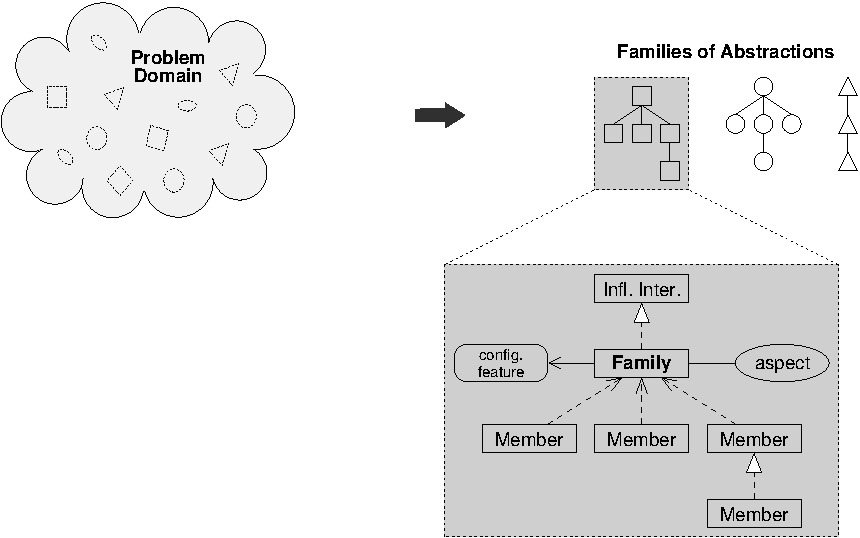
\includegraphics{fig/aosd-abs}}\par
%  \caption{Overview of application-oriented domain decomposition as
%    regards abstractions.\label{fig:aosd-abs}}
%\end{figure}

\begin{description}
\item[Families of scenario independent abstractions:] during domain
  decomposition, abstractions are identified from domain entities and
  grouped in families according to their commonalities. Yet during this
  phase, aspect separation is used to shape scenario-independent
  abstractions, thus enabling them to be reused in a variety of
  scenarios.  These abstractions are subsequently implemented to give
  rise to the actual software components.

%The implementation of the members of a family of abstractions is not
%restricted to the use of specialization as we would do in
%object-orientation, although it can occur, when convenient. For example,
%members could be implemented as classes conjunctly distributed as a
%package through aggregation or composition. Afterwards, some families
%may contain mutually exclusive members, that is, only one of the members
%can be present in the system configuration at a time.
  
\item[Scenario adapters:] as explained earlier in this article,
  Application-Oriented System Design dictates that scenario dependencies
  must be factored out as \emph{aspects}, thus keeping abstractions
  scena\-rio-independent.  However, for this strategy to work, means
  must be provided to apply factored aspects to abstractions in a
  transparent way. The traditional approach to do this would be
  deploying an \emph{aspect weaver}, though the \emph{scenario adapter}
  construct%~\cite{Froehlich:sci:2000}
  has the same potentialities without requiring an external tool.  A
  scenario adapter wraps an abstraction, intermediating its
  communication with scenario-dependent clients to perform the necessary
  scenario adaptations.
  
\item[Inflated interfaces:] summarize the features of all members of a
  family, creating a unique view of the family as a ``super component''.
  It allows application programmers to write their applications based on
  well-know, comprehensive interfaces, postponing the decision about
  which member of the family shall be use until enough configuration
  knowledge is acquired. The binding of an inflated interface to one of
  the members of a family can thus be made by automatic configuration
  tools that identify which features of the family were used in order to
  choose the simplest realization that implements the requested
  interface subset at compile-time.
\end{description}


\Section{Software Component Configuration}

An operating system designed according to the premises of
Application-Oriented System Design, besides all the benefits claimed by
software component engineering, has the additional advantage of being
suitable for automatic generation. The concept of inflated interface
enables an application-oriented operating system to be automatically
generated of out of a set of software components, since inflated
interfaces serve as a kind of requirement specification for the system
that must be generated.

An application written based on inflated interfaces can be submitted to
a tool that scans it searching for references to the interfaces, thus
rendering the features of each family that are necessary to support the
application at run-time. This task is accomplished by a tool, the
\texttt{analyzer}, that output an specification of requirements in the
form of partial component interface declarations, including methods,
types and constants that were used by the application.

The primary specification produced by the \texttt{analyzer} is
subsequently fed into a second tool, the \texttt{configurator}, that
consults a build-up database to further refine the specification.
This database holds information about each component in the
repository, as well as dependencies and composition rules that are
used by the \texttt{configurator} to build a dependency three.
Additionally, each component in the repository is tagged with a
``cost'' estimation, so that the \texttt{configurator} will chose
the ``cheapest'' option whenever two or more components satisfy a
dependency.  The output of the \texttt{configurator}
consists of a set of keys that define the binding of inflated
interfaces to abstractions and activate the scenario aspects and
configurable features eventually identified as necessary to satisfy
the constraints dictated by the target application or by the
configured execution scenario.

The last step in the generation process is accomplished by the
\texttt{generator}. This tool translates the keys produced by the
\texttt{configurator} into parameters for a statically metaprogramed
component framework and causes the compilation a tailored system
instance. %An overview of the whole procedure is depicted in
%figure~\ref{fig:tools}

%\begin{figure}[hbtp]
%  \centering\scalebox{0.5}{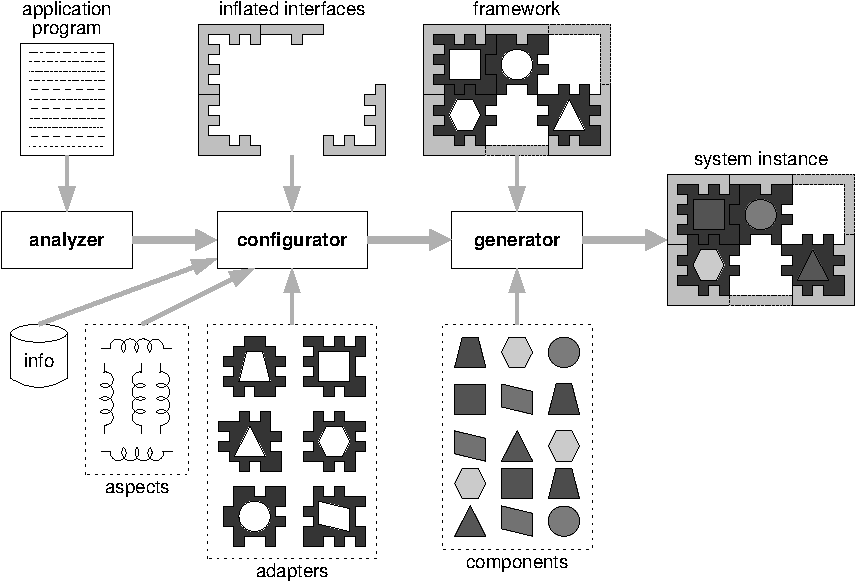
\includegraphics{fig/tools}}\par
%  \caption{An overview of the tools involved in automatic system
%  generation.\label{fig:tools}}
%\end{figure}


\Section{Software Component Description}

The strategy used to describe components in a repository and their
dependencies plays a key role in making the just described configuration
process possible.  The description of components must contain enough
information so that the \texttt{configurator} will be able to
automatically identify which abstractions better satisfy the
requirements of the application, and this without generating conflicts
or invalid configurations and compositions.

The strategy to describe components proposed here could indeed be taken
further as to specify components, for it encompasses much of the
information needed to implement components, including their interfaces
and relationships to other components. It is based on a declarative
language implemented around the \emph{Extensible Markup Language}~(XML)
and target at the description of individual families of
abstractions\footnote{A complete description of the software component
  repository is obtained simply by merging individual families'
  descriptions.}. The most significant elements in the language will be
explained next, taking as basis the corresponding \emph{Document Type
  Definition})~(DTD) fragments.

\SubSection{Families of abstractions}

The declaration of a family of abstractions in our language consists of
the family's inflated interface, an optional set of dependencies, and
optional set of traits, its common package and a set of family members
(software components), like this:

\inlineprg[DTD]{<!ELEMENT family (interface, common, member+,
  (feature, dependency, trait)* ) >}

The inflated interface of a family, as explained earlier, summarizes the
features of the whole family, %and is specified as follows:
%\inlineprg[DTD]{<!ELEMENT interface (type, constant, constructor, method)* >}
while the common package of a family holds type and constant declarations that
are common to all family members. %It is specified as:
%\inlineprg[DTD]{<!ELEMENT common (type, constant)* >}

The \textdtd{member} element shown bellow is used to describe each of
the members in a family. It is at the heart of the automatic
configuration process, enabling tools to make the proper selection while
looking for inflated interface realizations. A family member is declared
as:

\inlineprg[DTD]{<!ELEMENT member (super, type, constant,
constructor, method, trait, cost, feature, dependency)* >}

The \textdtd{super} element enables a member to inherit declarations of
other members in the family.%, allowing for the creation of incremental
%families much as in \emph{Incremental System Design}.
Elements \textdtd{type}, \textdtd{constant}, \textdtd{constructor} and
\textdtd{method} describe the interface of the member. A member's
interface designates a total or partial realization of the family's
inflated interface.  Element \textdtd{trait}, which can also be
specified for the family as whole, designates a configurable feature
that can be set by users, via configuration tools, in order to influence
the instantiation of a component %\footnote{Traits are made available at
%  compile-time to the static metaprograms that build up the component
%  framework.}.
A trait of a component can also be used to specify configuration
parameters that cannot be automatically figured out, such as the amount
of memory available on the target platform.

Additionally, each member of a family is tagged with a relative cost
estimation that is used by the configuration tools in case multiple
members satisfy the constraints to realize the family's inflated
interface in a given execution scenario. This cost estimation is
currently rather simplistic, consisting basically of an overhead
estimation made by the component developer. More sophisticate cost
models, including feed-back from the configuration tools, are planed for
the future.


\SubSection{Dependencies}

The description of the interfaces in a family of abstractions is the
main source of information for the proposed configuration tools, but
correctly assembling a component-based system goes far beyond the
verification of syntactic interface conformance: non-functional and
behavioral properties must also be conveyed. For this purpose, our
component description language includes two special elements:
\textdtd{feature} and \textdtd{dependency}. These elements can be
applied to virtually any other element in the language to specify
features provided by components and dependence among components that
cannot be directly deduced from their interfaces. Enriching the
description of components with features and dependencies can
significantly improve the correctness of the assembly process, helping
to avoid inconsistent component arrangements.

We have chosen a feature-based model to describe dependencies among
components.  To satisfy the dependencies, each family implements a
feature with the same name of the family, and each family's member
implements a feature with its same name. Families or members can also
implement aditional features using the \textdtd{feature} element. For
instance, consider a family of wireless network abstractions. Some
members could declare a ``reliable'' feature, making them eligible to
support an application whose execution scenario demands for reliable
communication. Similarly, members of a family of communication protocols
could specify the dependency on a ``reliable'' wireless network
infrastructure, while other could implement the feature themselves.

A feature has a name and, optionally, a value. The name should be
regarded as a meaningful feature in the application domain. Considering
the example above, we could specify the reliable feature of a wireless
network as follows:

\begin{lstlisting}[language=EPOSCFG,style=inlineprg]{}
<family name="Wireless_Network">
  <interface>...</interface>
  <member name="Wi-Fi">
    <feature name="reliable" />
  </member>
</family >
\end{lstlisting}

\noindent and the dependency in the protocol family as:

\begin{lstlisting}[language=EPOSCFG,style=inlineprg]{}
<family name="Wireless_Protocol">
  <interface>...</interface>
  <dependency feature="Wireless_Network" />
  <member name="Active_Message">
    <dependency feature="reliable" />
  </member>
</family >
\end{lstlisting}

It is important to mention that the fact of the \textxml{Active_Message}
member of the \textxml{Wireless_Protocol} family requiring a reliable
\textxml{Wireless_Network} does not summarily excludes members that do
not implement this feature: the \texttt{configurator} would first check
whether a scenario aspect is available that could be applied to a
non-reliable network in order to make it behave as a reliable one.


\Section{Supporting Tools}

At the present, we have prototype implementations of the
\texttt{analyzer} for applications written in \textsc{C++} and
\textsc{Java}. These tools are able to parse an input program and
produce a list of the system abstraction interfaces (inflated or
not) used by the program, identifying which methods have been
invoked and, in the case of \textsc{Java}, in which scope they have
been invoked.

This information serves as input for the \texttt{configurator}, which is
currently being developed. The \textsc{configurator} is indeed
implemented by two tools. The first one is responsible for executing the
algorithm that will select which members of each family will be included
in the customized version of the system. This algorithm consists in
reading the requirements found by the \texttt{analyzer} and compare them
with the interfaces of each member of the family as specified in the
repository.  Every time a new member is selected, its requirements are
recursively verified, including in the configuration any members from
other families that are needed to satisfy them. The second part of the
\texttt{configurator} is a graphical tool that allows the user to browse
an automatically generated configuration, making manual adjustments, if
needed. Moreover, the user will have to enter some important information
not discovered automatically: the configuration of the target machine
(architecture, processor, memory, etc.) and the values of the traits of
each component.

At last, the configuration keys outputted by the \texttt{configurator}
are used by the \texttt{generator}, which is implemented as a wrapper
for the \emph{GNU Compiler Collection}, to compile the system and
generate a boottable image.


%\Section{Further work}

%We are finishing the implementation of the \texttt{configurator} that
%will be capable of automatically generating the configuration for a
%customized version of \textsc{Epos}. Further works could refine the
%specification and implementation of the system configuration model in
%two aspects:

%\begin{itemize}
%\item Inclusion of behavioral specification in the component description
%  model. This specification would cover dependencies like: some method
%  of a component can only be invoked if the component is in determinate
%  state. This kind of specification would have to be validated by some
%  sort of formal mechanism, like a Prolog inference engine or a Petri
%  network.

%\item Evolution of the mechanism used to select members by performance.
%  Today, this task is accomplished using the specification by the
%  programmer of a cost estimate of each member on each family if the
%  form of overhead. More elaborated mechanisms would include an
%  automated way to measure real performance of each member during
%  execution time.
%\end{itemize}


\Section{Conclusion}

In this article we have presented an alternative to achieve automatic
run-time system generation taking as base a collection of software
components developed according with the Application-Oriented System
Design methodology. The proposed alternative consists of a novel
component description language and a set of configuration tools that are
able to automatically select and configure components to assembly an
application-oriented run-time support system.

The described configuration tools are in the final phase of development
and allows the exposition of the system libraries to application
programmers through a repository of reusable components described by
their inflated interfaces, which are automatically bound to a specific
realization at compile time. This is possible due to the component
specification model that contains all the information needed to generate
valid and optimized configurations for each application. This
architecture makes possible the creation of versions of the system
optimized for the target applications, assuring that the performance
levels and resource usage optimization will be within the levels
accepted by mobile applications.

\bibliographystyle{latex8}
\bibliography{guto,se,os,network}

\end{document}

%%% Local Variables:
%%% mode: latex
%%% TeX-master: "aiccsa2005"
%%% End:
